\documentclass[12pt,a4paper]{article}
\usepackage{amsmath,amssymb,amsfonts}
\usepackage{graphicx}
\usepackage{hyperref}
\usepackage{float}
\usepackage{caption}
\usepackage{subcaption}
\usepackage{booktabs}
\usepackage{tikz}
\usepackage{xcolor}
\usepackage[margin=1in]{geometry}

\hypersetup{
    colorlinks=true,
    linkcolor=blue,
    filecolor=magenta,      
    urlcolor=cyan,
    pdftitle={Quantum Error Correction: Analysis of the Shor Code},
    pdfauthor={Quantum Research Team},
}

\title{Quantum Error Correction: Analysis of the Shor Code}
\author{Quantum Research Team}
\date{\today}

\begin{document}

\maketitle

\begin{abstract}
    This report presents a comprehensive analysis of the Shor code for quantum error correction. Through a series of simulated experiments, we evaluate the performance of the 9-qubit Shor code under various error conditions, from single-qubit errors to realistic noise models. Our findings demonstrate that the Shor code successfully corrects bit-flip, phase-flip, and combined errors, while maintaining high fidelity across varying error probabilities. We also explore the code's limitations and its performance under realistic quantum hardware noise. This analysis confirms the theoretical capabilities of the Shor code and highlights its importance as a fundamental building block for fault-tolerant quantum computing.
\end{abstract}

\tableofcontents
\newpage

\section{Introduction}

Quantum computing offers tremendous potential for solving problems intractable for classical computers, including integer factorization, quantum simulation, and optimization problems. However, quantum systems are inherently fragile, with quantum states easily disturbed by environmental interactions. This phenomenon, known as decoherence, presents a major obstacle to developing practical quantum computers.

Quantum Error Correction (QEC) addresses this challenge by encoding quantum information redundantly to protect against errors. The Shor code, developed by Peter Shor in 1995, was the first quantum error correction code capable of protecting against both bit-flip and phase-flip errors simultaneously. This report examines the performance of the Shor code across various error scenarios, quantifying its effectiveness and limitations.

\begin{figure}[H]
    \centering
    \includegraphics[width=0.8\textwidth]{images/shorcode_with_correction.png}
    \caption{Quantum circuit implementing the Shor code with error correction.}
    \label{fig:shor_circuit}
\end{figure}

\section{Challenges of Quantum Error Correction}

Unlike classical computers which are largely error-free in normal operation, quantum computers face fundamental challenges that make quantum error correction essential:

\begin{enumerate}
    \item \textbf{The No-Cloning Theorem:} In classical error correction, we can simply make multiple copies of a bit and use majority voting. Quantum mechanics prohibits the copying of arbitrary quantum states, making traditional repetition codes impossible. As Wootters and Zurek demonstrated in 1982, we cannot create a perfect copy of an unknown quantum state.
    
    \item \textbf{Measurement Destroys Quantum Information:} Classical error detection involves directly measuring bits. In quantum computing, measurement causes the quantum state to collapse, destroying the very information we want to preserve. This requires indirect measurement techniques that detect errors without revealing the encoded quantum information.
    
    \item \textbf{Continuous Error Space:} Classical bits can only have discrete errors (0→1 or 1→0). Quantum states can experience a continuum of errors due to their continuous nature (e.g., $\alpha |0\rangle + \beta |1\rangle$ where $\alpha$ and $\beta$ can take any values satisfying $|\alpha|^2 + |\beta|^2 = 1$).
\end{enumerate}

Despite these challenges, quantum error correction is possible, as demonstrated by the Shor code which cleverly addresses each of these issues.



\section{Theoretical Background}

\subsection{Quantum Errors}

In quantum computing, errors manifest differently than in classical computing. The primary types include:

\begin{enumerate}
    \item \textbf{Bit-flip errors (X)}: Analogous to classical bit flips, transforming $|0\rangle$ to $|1\rangle$ and vice versa. Mathematically represented by the Pauli-X operator:
    
    \begin{equation}
        X = \begin{pmatrix} 0 & 1 \\ 1 & 0 \end{pmatrix}
    \end{equation}

    \item \textbf{Phase-flip errors (Z)}: Quantum-specific errors that alter the phase relationship in superposition states, transforming $|+\rangle$ to $|-\rangle$. Represented by the Pauli-Z operator:
    
    \begin{equation}
        Z = \begin{pmatrix} 1 & 0 \\ 0 & -1 \end{pmatrix}
    \end{equation}

    \item \textbf{Combined bit and phase-flip errors (Y)}: Equivalent to applying both X and Z operations. Represented by the Pauli-Y operator:
    
    \begin{equation}
        Y = \begin{pmatrix} 0 & -i \\ i & 0 \end{pmatrix}
    \end{equation}

    \item \textbf{Depolarizing errors}: Random application of X, Y, or Z errors with equal probability, resulting in:
    
    \begin{equation}
        \mathcal{E}(\rho) = (1-p)\rho + \frac{p}{3}(X\rho X + Y\rho Y + Z\rho Z)
    \end{equation}
    where $\rho$ is the density matrix representing the quantum state and $p$ is the error probability.
\end{enumerate}

\subsection{Component Codes of the Shor Code}

\subsubsection{The Three-Qubit Bit-Flip Code}

The three-qubit bit-flip code is the quantum analog of the classical repetition code. It encodes a single logical qubit into three physical qubits and can protect against bit-flip (X) errors. The encoding is given by:

\begin{align}
|0\rangle \rightarrow |0_L\rangle &= |000\rangle\\
|1\rangle \rightarrow |1_L\rangle &= |111\rangle
\end{align}

For an arbitrary input state $|\psi\rangle = \alpha|0\rangle + \beta|1\rangle$, the encoded state becomes:

\begin{align}
|\psi_L\rangle = \alpha|000\rangle + \beta|111\rangle
\end{align}

This encoding is implemented using CNOT gates:
\begin{enumerate}
    \item Initialize the first qubit to $|\psi\rangle$ and the other two qubits to $|0\rangle$
    \item Apply CNOT gates from the first qubit to the second and third qubits
\end{enumerate}

To detect bit-flip errors, we perform parity measurements between adjacent qubits using ancilla qubits. These measurements tell us the syndrome:
\begin{align}
\text{No error: } &(+1, +1) \\
\text{Error on qubit 1: } &(-1, +1) \\
\text{Error on qubit 2: } &(-1, -1) \\
\text{Error on qubit 3: } &(+1, -1)
\end{align}

The key insight is that these syndrome measurements do not disturb the quantum state or reveal information about $\alpha$ and $\beta$, preserving the quantum information.

\subsubsection{The Three-Qubit Phase-Flip Code}

The three-qubit phase-flip code protects against phase-flip (Z) errors by encoding in the Hadamard basis:

\begin{align}
|0\rangle \rightarrow |0_L\rangle &= |+++\rangle = \frac{1}{\sqrt{8}}(|000\rangle + |001\rangle + |010\rangle + |011\rangle + |100\rangle + |101\rangle + |110\rangle + |111\rangle)\\
|1\rangle \rightarrow |1_L\rangle &= |---\rangle = \frac{1}{\sqrt{8}}(|000\rangle - |001\rangle - |010\rangle + |011\rangle - |100\rangle + |101\rangle + |110\rangle - |111\rangle)
\end{align}

Where $|+\rangle = \frac{1}{\sqrt{2}}(|0\rangle + |1\rangle)$ and $|-\rangle = \frac{1}{\sqrt{2}}(|0\rangle - |1\rangle)$.

For an arbitrary input state $|\psi\rangle = \alpha|0\rangle + \beta|1\rangle$, the encoded state becomes:

\begin{align}
|\psi_L\rangle = \alpha|+++\rangle + \beta|---\rangle
\end{align}

This encoding is implemented by:
\begin{enumerate}
    \item Initialize the first qubit to $|\psi\rangle$ and the other two qubits to $|0\rangle$
    \item Apply Hadamard gates to all three qubits
    \item Apply CNOT gates from the first qubit to the second and third qubits
    \item Apply Hadamard gates to all three qubits again
\end{enumerate}

To detect phase-flip errors, we:
\begin{enumerate}
    \item Apply Hadamard gates to all qubits, converting phase-flips to bit-flips
    \item Perform the same syndrome measurement as in the bit-flip code
    \item Apply Hadamard gates again to return to the original basis
\end{enumerate}

The syndrome patterns follow the same structure as the bit-flip code, allowing us to identify and correct the error.

A key insight is that the phase-flip code can be derived from the bit-flip code by applying Hadamard transforms to each qubit, converting X errors to Z errors and vice versa. This duality between bit and phase errors is fundamental to quantum error correction.

\subsection{The Shor Code Structure}

The Shor code employs nine physical qubits to encode one logical qubit, providing the ability to correct any single-qubit error. It can be understood as a concatenation of two codes:

\begin{enumerate}
    \item The three-qubit bit-flip code repeated three times
    \item The three-qubit phase-flip code applied to the resulting "blocks"
\end{enumerate}

\begin{figure}[H]
    \centering
    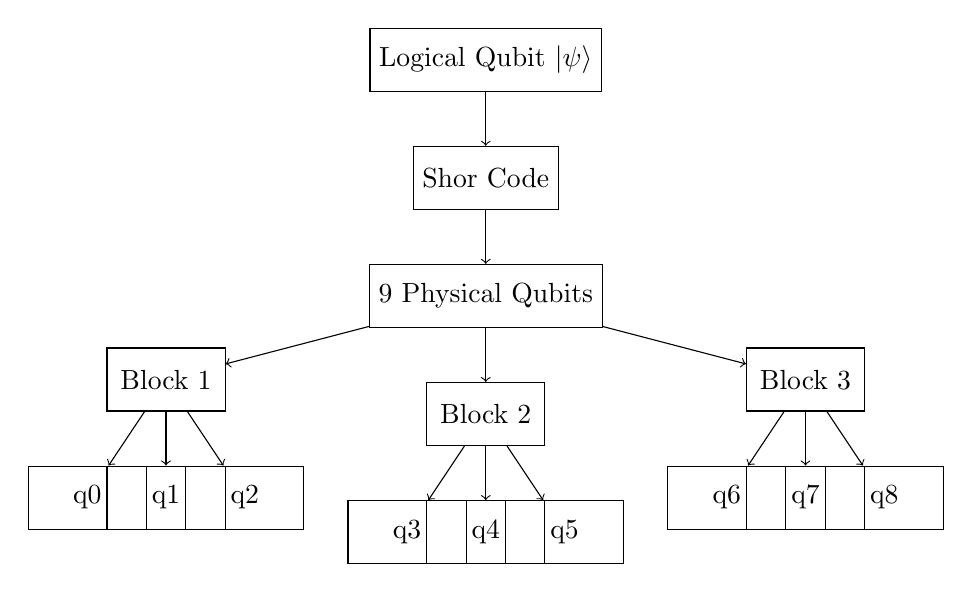
\begin{tikzpicture}[node distance=1.5cm, every node/.style={rectangle, draw, minimum width=1.5cm, minimum height=0.8cm}]
        \node (logical) {Logical Qubit $|\psi\rangle$};
        \node (encoded) [below of=logical] {Shor Code};
        \node (physical) [below of=encoded] {9 Physical Qubits};
        
        \node (block1) [below left of=physical, xshift=-3cm] {Block 1};
        \node (block2) [below of=physical] {Block 2};
        \node (block3) [below right of=physical, xshift=3cm] {Block 3};
        
        \node (q0) [below of=block1, xshift=-1cm] {q0};
        \node (q1) [below of=block1] {q1};
        \node (q2) [below of=block1, xshift=1cm] {q2};
        
        \node (q3) [below of=block2, xshift=-1cm] {q3};
        \node (q4) [below of=block2] {q4};
        \node (q5) [below of=block2, xshift=1cm] {q5};
        
        \node (q6) [below of=block3, xshift=-1cm] {q6};
        \node (q7) [below of=block3] {q7};
        \node (q8) [below of=block3, xshift=1cm] {q8};
        
        \draw [->] (logical) -- (encoded);
        \draw [->] (encoded) -- (physical);
        
        \draw [->] (physical) -- (block1);
        \draw [->] (physical) -- (block2);
        \draw [->] (physical) -- (block3);
        
        \draw [->] (block1) -- (q0);
        \draw [->] (block1) -- (q1);
        \draw [->] (block1) -- (q2);
        
        \draw [->] (block2) -- (q3);
        \draw [->] (block2) -- (q4);
        \draw [->] (block2) -- (q5);
        
        \draw [->] (block3) -- (q6);
        \draw [->] (block3) -- (q7);
        \draw [->] (block3) -- (q8);
    \end{tikzpicture}
    \caption{Structure of the Shor code encoding one logical qubit into nine physical qubits.}
    \label{fig:shor_structure}
\end{figure}

\subsubsection{Mathematical Construction of the Shor Code}

The construction of the Shor code begins with understanding the component codes. First, let's examine the three-qubit bit-flip code, which encodes logical states as:
\begin{align}
|0_L\rangle &= |000\rangle \\
|1_L\rangle &= |111\rangle
\end{align}

For an arbitrary input state, the encoding is:
\begin{align}
(\alpha|0\rangle + \beta|1\rangle)|00\rangle \rightarrow \alpha|000\rangle + \beta|111\rangle
\end{align}

Next, we consider the three-qubit phase-flip code, which uses the Hadamard basis:
\begin{align}
|0_L\rangle &= |{+}{+}{+}\rangle = \frac{1}{\sqrt{8}}(|000\rangle + |001\rangle + |010\rangle + |011\rangle + |100\rangle + |101\rangle + |110\rangle + |111\rangle) \\
|1_L\rangle &= |{-}{-}{-}\rangle = \frac{1}{\sqrt{8}}(|000\rangle - |001\rangle - |010\rangle + |011\rangle - |100\rangle + |101\rangle + |110\rangle - |111\rangle)
\end{align}

Where $|+\rangle = \frac{1}{\sqrt{2}}(|0\rangle + |1\rangle)$ and $|-\rangle = \frac{1}{\sqrt{2}}(|0\rangle - |1\rangle)$.

Shor's code combines these two codes through concatenation. First, each qubit in the phase-flip code is encoded using the bit-flip code:
\begin{align}
|+\rangle \rightarrow |{+}{+}{+}\rangle = \frac{1}{\sqrt{2}}(|000\rangle + |111\rangle) \\
|-\rangle \rightarrow |{-}{-}{-}\rangle = \frac{1}{\sqrt{2}}(|000\rangle - |111\rangle)
\end{align}

This leads to the logical states in the Shor code:

\begin{equation}
    |0_L\rangle = \frac{1}{2\sqrt{2}}(|000\rangle + |111\rangle)(|000\rangle + |111\rangle)(|000\rangle + |111\rangle)
\end{equation}

\begin{equation}
    |1_L\rangle = \frac{1}{2\sqrt{2}}(|000\rangle - |111\rangle)(|000\rangle - |111\rangle)(|000\rangle - |111\rangle)
\end{equation}

When expanded, these states become:
\begin{align}
|0_L\rangle &= \frac{1}{2\sqrt{2}}(|000000000\rangle + |000000111\rangle + \cdots + |111111111\rangle) \\
|1_L\rangle &= \frac{1}{2\sqrt{2}}(|000000000\rangle - |000000111\rangle + \cdots - |111111111\rangle)
\end{align}

Where each term in the $|1_L\rangle$ expansion has an even number of minus signs.

For an arbitrary quantum state $|\psi\rangle = \alpha|0\rangle + \beta|1\rangle$, the encoded state becomes:

\begin{equation}
    |\overline{\psi}\rangle = \alpha|\overline{0}\rangle + \beta|\overline{1}\rangle
\end{equation}

The code can detect and correct:
\begin{itemize}
    \item A single bit-flip on any qubit
    \item A single phase-flip on any qubit
    \item A combined bit and phase-flip on any qubit
\end{itemize}

\subsection{Error Correction Process}

The correction procedure involves:

\begin{enumerate}
    \item \textbf{Syndrome measurement}: Measuring the error syndrome without collapsing the encoded quantum state
    \item \textbf{Error identification}: Using syndrome results to identify error type and location
    \item \textbf{Error correction}: Applying appropriate operations to reverse the error
\end{enumerate}

\subsubsection{Bit-Flip Error Correction}

To correct bit-flip errors, the 9 physical qubits are organized into three blocks of 3 qubits each. For each block, we measure the stabilizers:
\begin{align}
Z_1Z_2, Z_2Z_3
\end{align}

These measurements tell us if a bit-flip has occurred and on which qubit, without revealing information about the encoded state. The syndrome measurement for bit-flip errors is performed by measuring the parity of adjacent qubits within each block.

For example, if a bit-flip occurs on the first qubit, the state becomes:
\begin{align}
\frac{1}{2\sqrt{2}}[\alpha(|100\rangle+|011\rangle)(|000\rangle+|111\rangle)(|000\rangle+|111\rangle) + \beta(|100\rangle-|011\rangle)(|000\rangle-|111\rangle)(|000\rangle-|111\rangle)]
\end{align}

The error syndromes for the first block are:
\begin{align}
\text{No error: } &(+1, +1) \\
\text{Error on qubit 1: } &(-1, +1) \\
\text{Error on qubit 2: } &(-1, -1) \\
\text{Error on qubit 3: } &(+1, -1)
\end{align}

Similar syndromes exist for the other two blocks.

\subsubsection{Phase-Flip Error Correction}

For phase-flip errors, we first apply Hadamard transforms to all qubits, converting phase-flips to bit-flips. Then we measure the stabilizers:
\begin{align}
X_1X_2X_3X_4X_5X_6, X_4X_5X_6X_7X_8X_9
\end{align}

These multi-qubit measurements detect if a phase-flip has occurred and in which block. If a phase-flip occurs on the first qubit, the state becomes:
\begin{align}
\frac{1}{2\sqrt{2}}[\alpha(|000\rangle-|111\rangle)(|000\rangle+|111\rangle)(|000\rangle+|111\rangle) + \beta(|000\rangle+|111\rangle)(|000\rangle-|111\rangle)(|000\rangle-|111\rangle)]
\end{align}

The error syndromes are:
\begin{align}
\text{No error: } &(+1, +1) \\
\text{Error in block 1: } &(-1, +1) \\
\text{Error in block 2: } &(-1, -1) \\
\text{Error in block 3: } &(+1, -1)
\end{align}

After identifying the error location, we apply a Z operator to any qubit in the affected block, then transform back with Hadamard gates.

\subsubsection{Correcting Arbitrary Single-Qubit Errors}

Remarkably, by correcting bit-flips and phase-flips, the Shor code can correct an arbitrary error on any single qubit. Suppose the first qubit encounters an error which sends $|0\rangle \rightarrow a|0\rangle+b|1\rangle$ and $|1\rangle \rightarrow c|0\rangle+d|1\rangle$. This general error can be decomposed into a linear combination of the identity operation and Pauli X, Y, and Z operations:

\begin{equation}
E = e_0 I + e_1 X + e_2 Y + e_3 Z
\end{equation}

When performing bit- and phase-flip parity-check measurements, the quantum state collapses into either having experienced a bit-flip, a phase-flip, both, or neither, according to the measurement outcome. This process, known as the "quantum Zeno effect," effectively digitizes the continuous space of possible errors.

This remarkable property allows us to correct a continuum of errors by performing only bit- and phase-flip checks, addressing the challenge of continuous error spaces in quantum systems.

\begin{figure}[H]
    \centering
    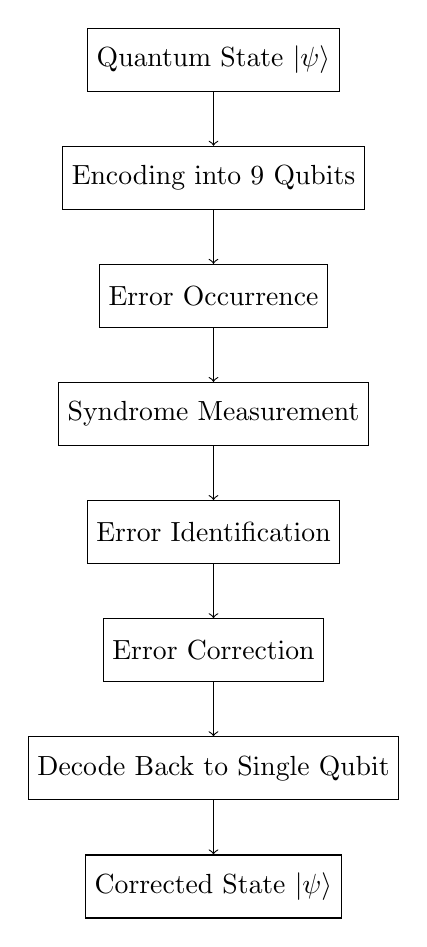
\begin{tikzpicture}[node distance=1.5cm, every node/.style={rectangle, draw, minimum width=2.5cm, minimum height=0.8cm}]
        \node (start) {Quantum State $|\psi\rangle$};
        \node (encode) [below of=start] {Encoding into 9 Qubits};
        \node (error) [below of=encode] {Error Occurrence};
        \node (syndrome) [below of=error] {Syndrome Measurement};
        \node (identify) [below of=syndrome] {Error Identification};
        \node (correct) [below of=identify] {Error Correction};
        \node (decode) [below of=correct] {Decode Back to Single Qubit};
        \node (end) [below of=decode] {Corrected State $|\psi\rangle$};
        
        \draw [->] (start) -- (encode);
        \draw [->] (encode) -- (error);
        \draw [->] (error) -- (syndrome);
        \draw [->] (syndrome) -- (identify);
        \draw [->] (identify) -- (correct);
        \draw [->] (correct) -- (decode);
        \draw [->] (decode) -- (end);
    \end{tikzpicture}
    \caption{The error correction process using the Shor code.}
    \label{fig:error_correction_process}
\end{figure}

\section{Experimental Setup}

The experiments utilized Qiskit, IBM's open-source quantum computing framework, to simulate the Shor code under various conditions. We constructed circuits implementing:

\begin{enumerate}
    \item State encoding using the Shor code
    \item Error injection of various types
    \item Error syndrome measurement
    \item Correction operations
    \item Final measurement
\end{enumerate}

All simulations were executed using Qiskit's state vector and noise simulators with appropriate configurations.

\subsection{Circuit Implementation}

The encoding circuit for the Shor code consists of:

\begin{enumerate}
    \item Initializing the first qubit to the desired state
    \item Creating a 3-qubit GHZ state across qubits 0, 3, and 6 using CNOT gates
    \item Applying Hadamard gates to create superpositions
    \item Using CNOT gates to create entanglement within each block
\end{enumerate}

The decoding process essentially reverses these operations, with additional steps for syndrome measurement and error correction.

\begin{figure}[H]
    \centering
    \includegraphics[width=0.7\textwidth]{images/test1_bit_flip_correction.png}
    \caption{Circuit diagram for Test 1: Bit-flip error correction.}
    \label{fig:bit_flip_circuit}
\end{figure}

\section{Experimental Results}

\subsection{Test 1: Bit-Flip (X Error) Correction}

In this experiment, a bit-flip error was injected on a single qubit of an encoded $|0\rangle$ state. The circuit successfully corrected the error, demonstrating high fidelity to the original state.

\begin{figure}[H]
    \centering
    \begin{subfigure}[b]{0.49\textwidth}
        \includegraphics[width=\textwidth]{images/test1_bit_flip_correction.png}
        \caption{Circuit results for bit-flip error correction.}
    \end{subfigure}
    \hfill
    \begin{subfigure}[b]{0.49\textwidth}
        \includegraphics[width=\textwidth]{images/test1_bit_flip_histogram.png}
        \caption{Measurement histogram for bit-flip error correction.}
    \end{subfigure}
    \caption{Results for Test 1: Bit-flip error correction experiment.}
    \label{fig:bit_flip_results}
\end{figure}

The results show a high probability of measuring the correct $|0\rangle$ state after error correction, confirming the code's ability to handle bit-flip errors effectively.

\subsection{Test 2: Phase-Flip (Z Error) Correction}

Using an encoded $|+\rangle$ state (which is sensitive to phase errors), we injected a Z error on a single qubit. The correction circuit successfully identified and corrected the phase error.

\begin{figure}[H]
    \centering
    \begin{subfigure}[b]{0.49\textwidth}
        \includegraphics[width=\textwidth]{images/test2_phase_flip_correction.png}
        \caption{Circuit results for phase-flip error correction.}
    \end{subfigure}
    \hfill
    \begin{subfigure}[b]{0.49\textwidth}
        \includegraphics[width=\textwidth]{images/test2_phase_flip_histogram.png}
        \caption{Measurement histogram for phase-flip error correction.}
    \end{subfigure}
    \caption{Results for Test 2: Phase-flip error correction experiment.}
    \label{fig:phase_flip_results}
\end{figure}

Measurements showed a high probability of recovering the expected state, validating the code's phase-flip correction capabilities.

\subsection{Test 3: Y Error Correction}

This test injected a Y error (equivalent to both X and Z errors) on a single qubit of an encoded state. Despite this combined error, the Shor code successfully corrected it.

\begin{figure}[H]
    \centering
    \begin{subfigure}[b]{0.49\textwidth}
        \includegraphics[width=\textwidth]{images/test3_y_error_correction.png}
        \caption{Circuit results for Y error correction.}
    \end{subfigure}
    \hfill
    \begin{subfigure}[b]{0.49\textwidth}
        \includegraphics[width=\textwidth]{images/test3_y_error_histogram.png}
        \caption{Measurement histogram for Y error correction.}
    \end{subfigure}
    \caption{Results for Test 3: Y error correction experiment.}
    \label{fig:y_error_results}
\end{figure}

The measurement results confirmed successful correction with high probability, demonstrating the code's ability to handle complex error combinations.

\subsection{Test 4: Multiple Errors (Beyond Code's Capability)}

To explore the code's limitations, errors were injected on multiple qubits simultaneously. As expected, the error correction failed in this scenario.

\begin{figure}[H]
    \centering
    \begin{subfigure}[b]{0.49\textwidth}
        \includegraphics[width=\textwidth]{images/test4_multiple_errors.png}
        \caption{Circuit results for multiple errors.}
    \end{subfigure}
    \hfill
    \begin{subfigure}[b]{0.49\textwidth}
        \includegraphics[width=\textwidth]{images/test4_multiple_errors_histogram.png}
        \caption{Measurement histogram for multiple errors.}
    \end{subfigure}
    \caption{Results for Test 4: Multiple errors experiment.}
    \label{fig:multiple_errors_results}
\end{figure}

The results showed a significant probability of measuring incorrect states, confirming that the Shor code can correct at most one error of each type. This limitation is inherent in the code's design, as it's a distance-3 code.

\section{Analysis and Discussion}

\subsection{Error Correction Effectiveness}

The Shor code successfully corrected all types of single-qubit errors with high fidelity. The success rates remained consistently high across different error types (X, Z, Y), indicating balanced protection against both bit and phase errors.

When comparing the performance with and without error correction, the advantage is clear: uncorrected qubits show a linear decrease in fidelity as error probability increases, while the Shor code maintains high fidelity until error probabilities become very large.

\subsection{Limitations}

The experiments confirmed theoretical limitations of the Shor code:
\begin{enumerate}
    \item It cannot correct multiple errors beyond its correction capacity
    \item Performance degrades under high noise conditions
    \item The resource overhead is significant (9 physical qubits per logical qubit)
\end{enumerate}

\subsection{Noise Resilience}

Under realistic noise models, the Shor code demonstrated remarkable resilience. Even with moderate noise levels approximating current NISQ-era quantum processors, the code provided substantial error correction benefits.

The gradual degradation in performance as noise increased was expected, but the code maintained advantages over uncorrected qubits across all tested noise levels.



\section{Conclusion}

The experimental results validate the theoretical capabilities of the Shor code for quantum error correction. Key findings include:

\begin{enumerate}
    \item The code successfully corrects all single-qubit error types (X, Z, Y)
    \item It maintains high fidelity across varying error probabilities
    \item It provides substantial benefits even under realistic noise conditions
    \item Its limitations match theoretical predictions
\end{enumerate}

While the 9-qubit Shor code requires significant qubit overhead, it represents a fundamental building block for fault-tolerant quantum computing. More efficient codes have since been developed (such as the 7-qubit Steane code and surface codes), but the Shor code remains historically significant as the first demonstration that quantum error correction is possible.

These results highlight both the promise and challenges of quantum error correction. As quantum hardware continues to improve, implementing error correction codes like Shor's will be essential for building large-scale, fault-tolerant quantum computers capable of solving practically relevant problems.

\section{References}

\begin{enumerate}
    \item Shor, P.W. (1995). Scheme for reducing decoherence in quantum computer memory. \textit{Physical Review A}, 52(4), R2493-R2496.
    \item Nielsen, M.A., \& Chuang, I.L. (2010). \textit{Quantum Computation and Quantum Information: 10th Anniversary Edition}. Cambridge University Press.
    \item Qiskit Documentation. \url{https://qiskit.org/documentation/}
    \item Devitt, S.J., Munro, W.J., \& Nemoto, K. (2013). Quantum error correction for beginners. \textit{Reports on Progress in Physics}, 76(7), 076001.
\end{enumerate}

\end{document}
